\begin{figure}[htb]
  \begin{center}
    \resizebox{\textwidth}{!}{
      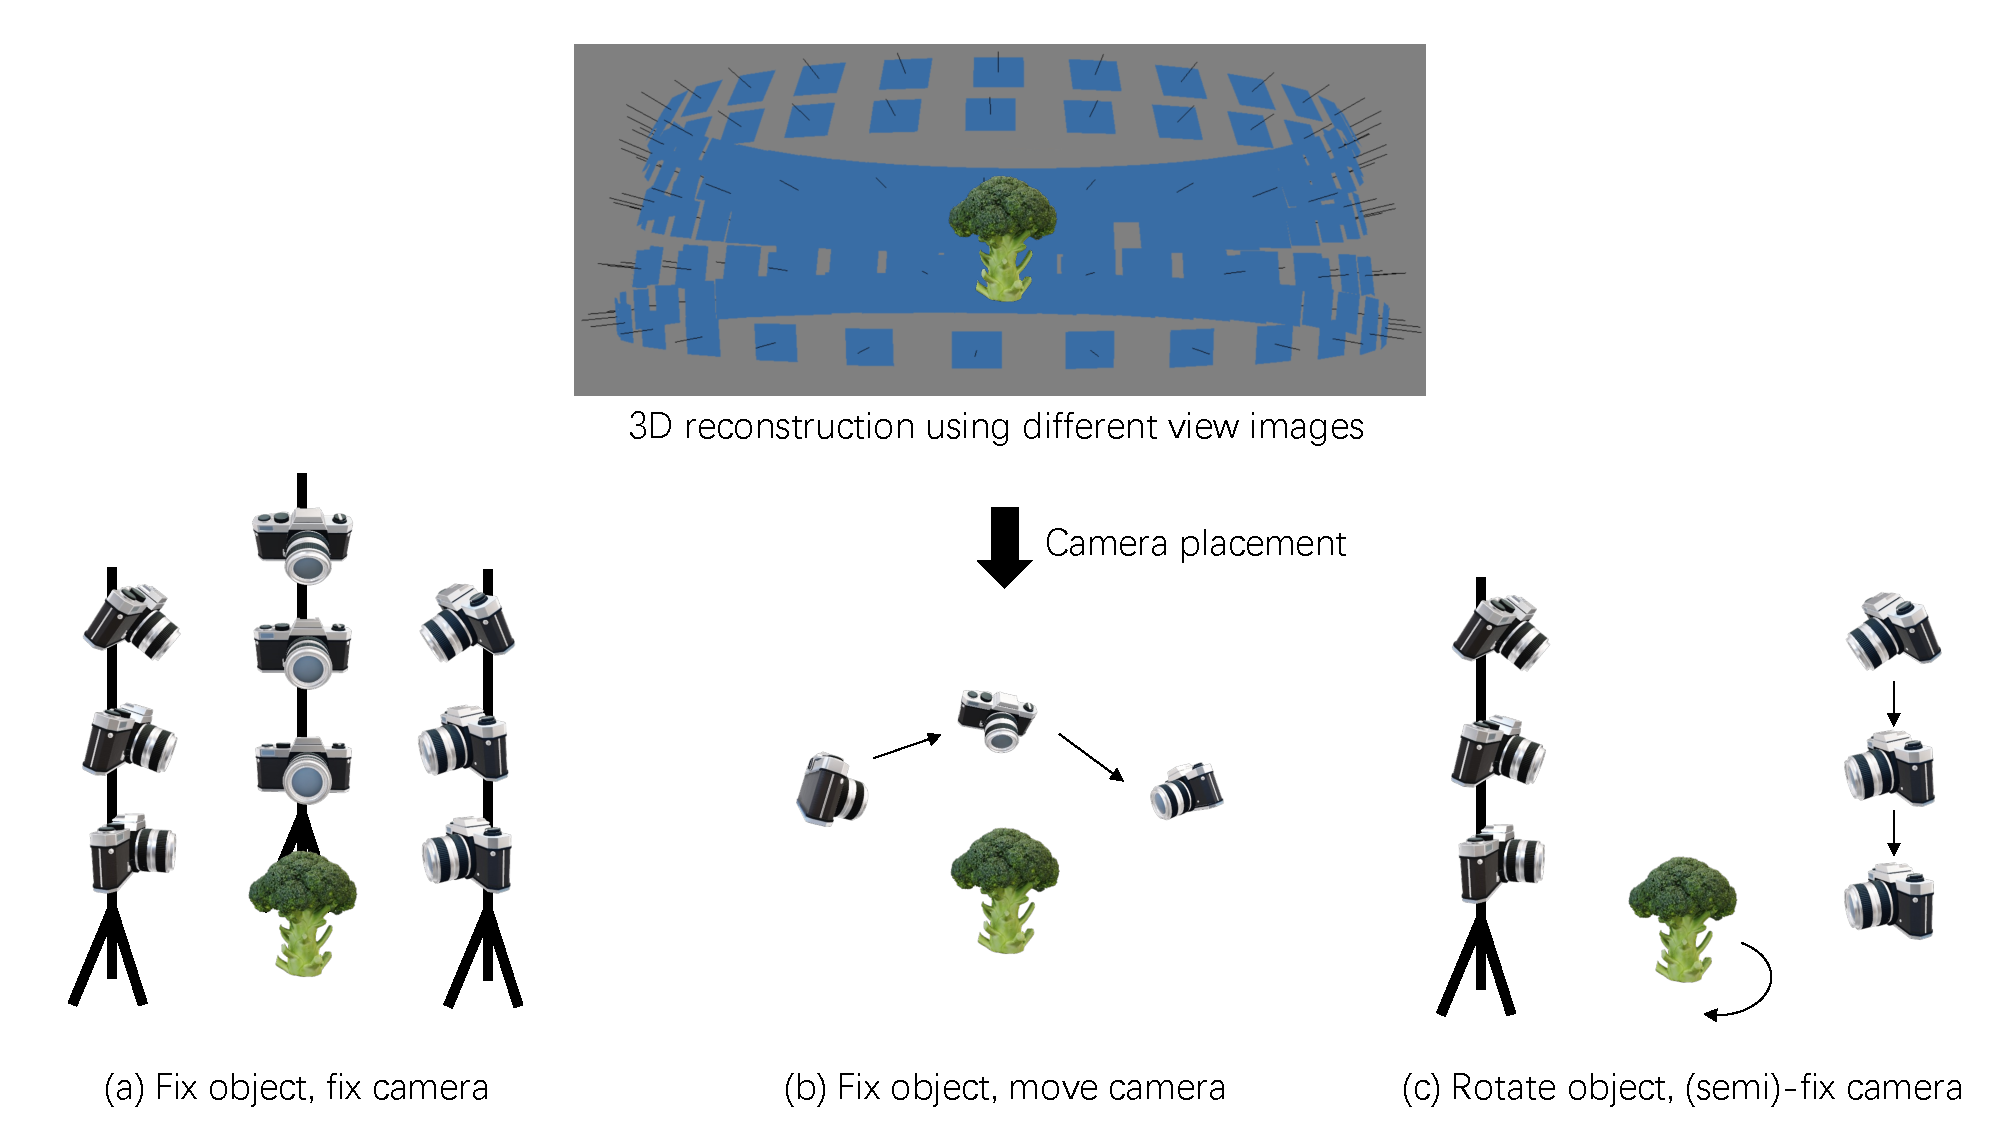
\includegraphics{figures/des/sfm_types.pdf}
    }
  \end{center}
  \caption[Current photogrammetry (3D reconstruction) methods]{
    The current camera placement for 3D reconstruction. (a) fixing the object and taking images using multiple fixed cameras at the same time, also called forward intersection; (b) fixing the object but taking images by using a moved camera, also called backward resection; (c) rotating the object and taking images using fewer multiple fixed cameras, or a camera fixed at different locations for each rotation.
  }
  \label{fig:des1}
\end{figure}